\chapter{Algorytm rozwiązania}\label{chap:solution_algorithm}

\begin{figure}[H]    
    \centering
    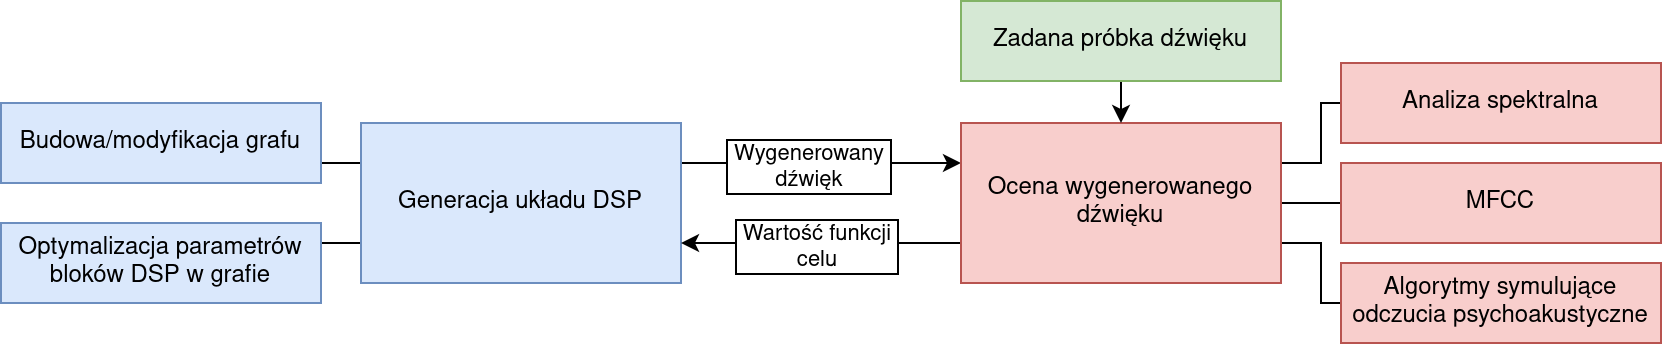
\includegraphics[width=1.0\linewidth]{rys04/solution_algorithm_diagram.png}
    \caption{
      Diagram algorytmu rozwiązania zaimplementowanego w ramach pracy.
      Algorytm oceny może wykorzystywać różne funkcje celu, finalnie zastosowano
      MFCC oraz \textit{dynamic time wrapping},
      proces wyboru funkcji celu opisuje rozdział~\ref{target_function_chapter}.
    }\label{fig:solution_algorithm_diagram}
\end{figure}

Jak opisano w rozdziale poświęconym definicji problemu~(\ref{chap:problem_definition}), praca
rozwiązuje problem budowy grafu DSP z wykorzystaniem dwóch algorytmów:
\begin{enumerate}
  \item Algorytm generujący graf DSP, opisany w rozdziale~\ref{dsp_graph_chapter},
  \item Algorytm oceniający jak bardzo wygenerowany dźwięk jest bliski dźwiękowi docelowemu pod względem barwy,
    opisany w rozdziale~\ref{target_function_chapter}.
\end{enumerate}

Praca wykorzystuje algorytm genetyczny, w którym genotyp odpowiada za
strukturę grafu~\ref{fig:example_generated_graph} oraz wartości
przypisane do parametrów grafu~(\ref{eq:graph_structure_generation_function},~\ref{eq:graph_params_assignment}).
% Diagram blokowy~\ref{fig:solution_algorithm_diagram} ilustruje zaimplementowany algorytm.
Algorytm generuje różne warianty grafów przetwarzania sygnałów powszechnie
wykorzystywane w syntezatorach dźwięku~\cite{minilogue_diagram}~\cite{digitone_manual}~\cite{yamaha_dx7_manual}.
Takie podejście pozwala na dostosowanie grafu do danego rodzaju syntezy,
lub połączenie wielu typów syntezy w celu uzyskania bardziej złożonego brzmienia.
Algorytm wybiera węzły dla każdej sekcji
zilustrowanej na rysunku~\ref{fig:synth_architecture_diagram}.

\begin{figure}[H]
    \centering
    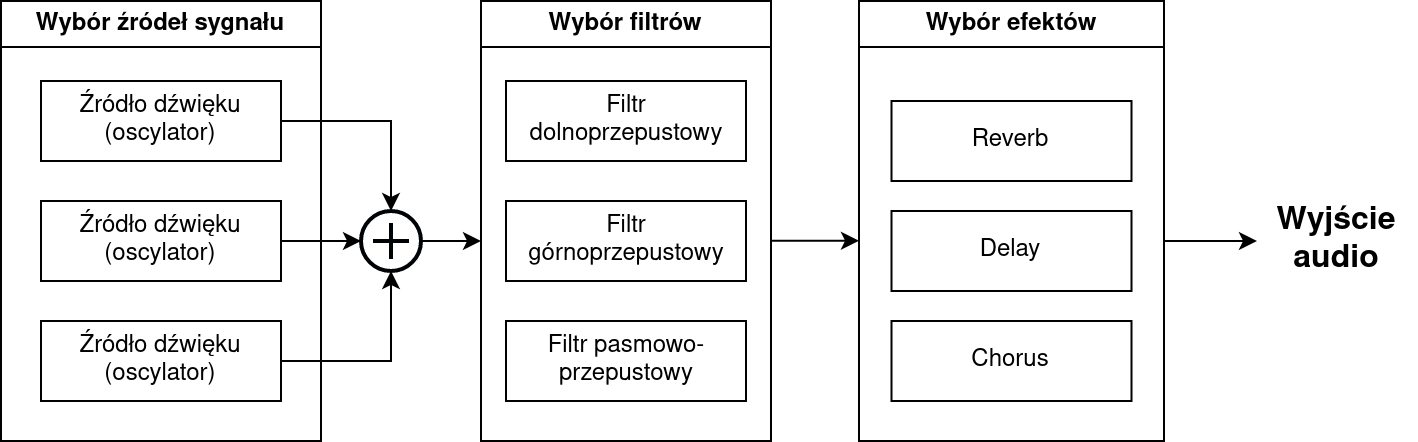
\includegraphics[width=0.8\linewidth]{rys06/synth_architecture.png}
    \caption{
      Sekcje przetwarzania sygnałów oraz przykładowe węzły przetwarzania
      sygnałów, które są w nich powszechnie wykorzystywane.
    }\label{fig:synth_architecture_diagram}
\end{figure}

\begin{figure}[H]
    \centering
    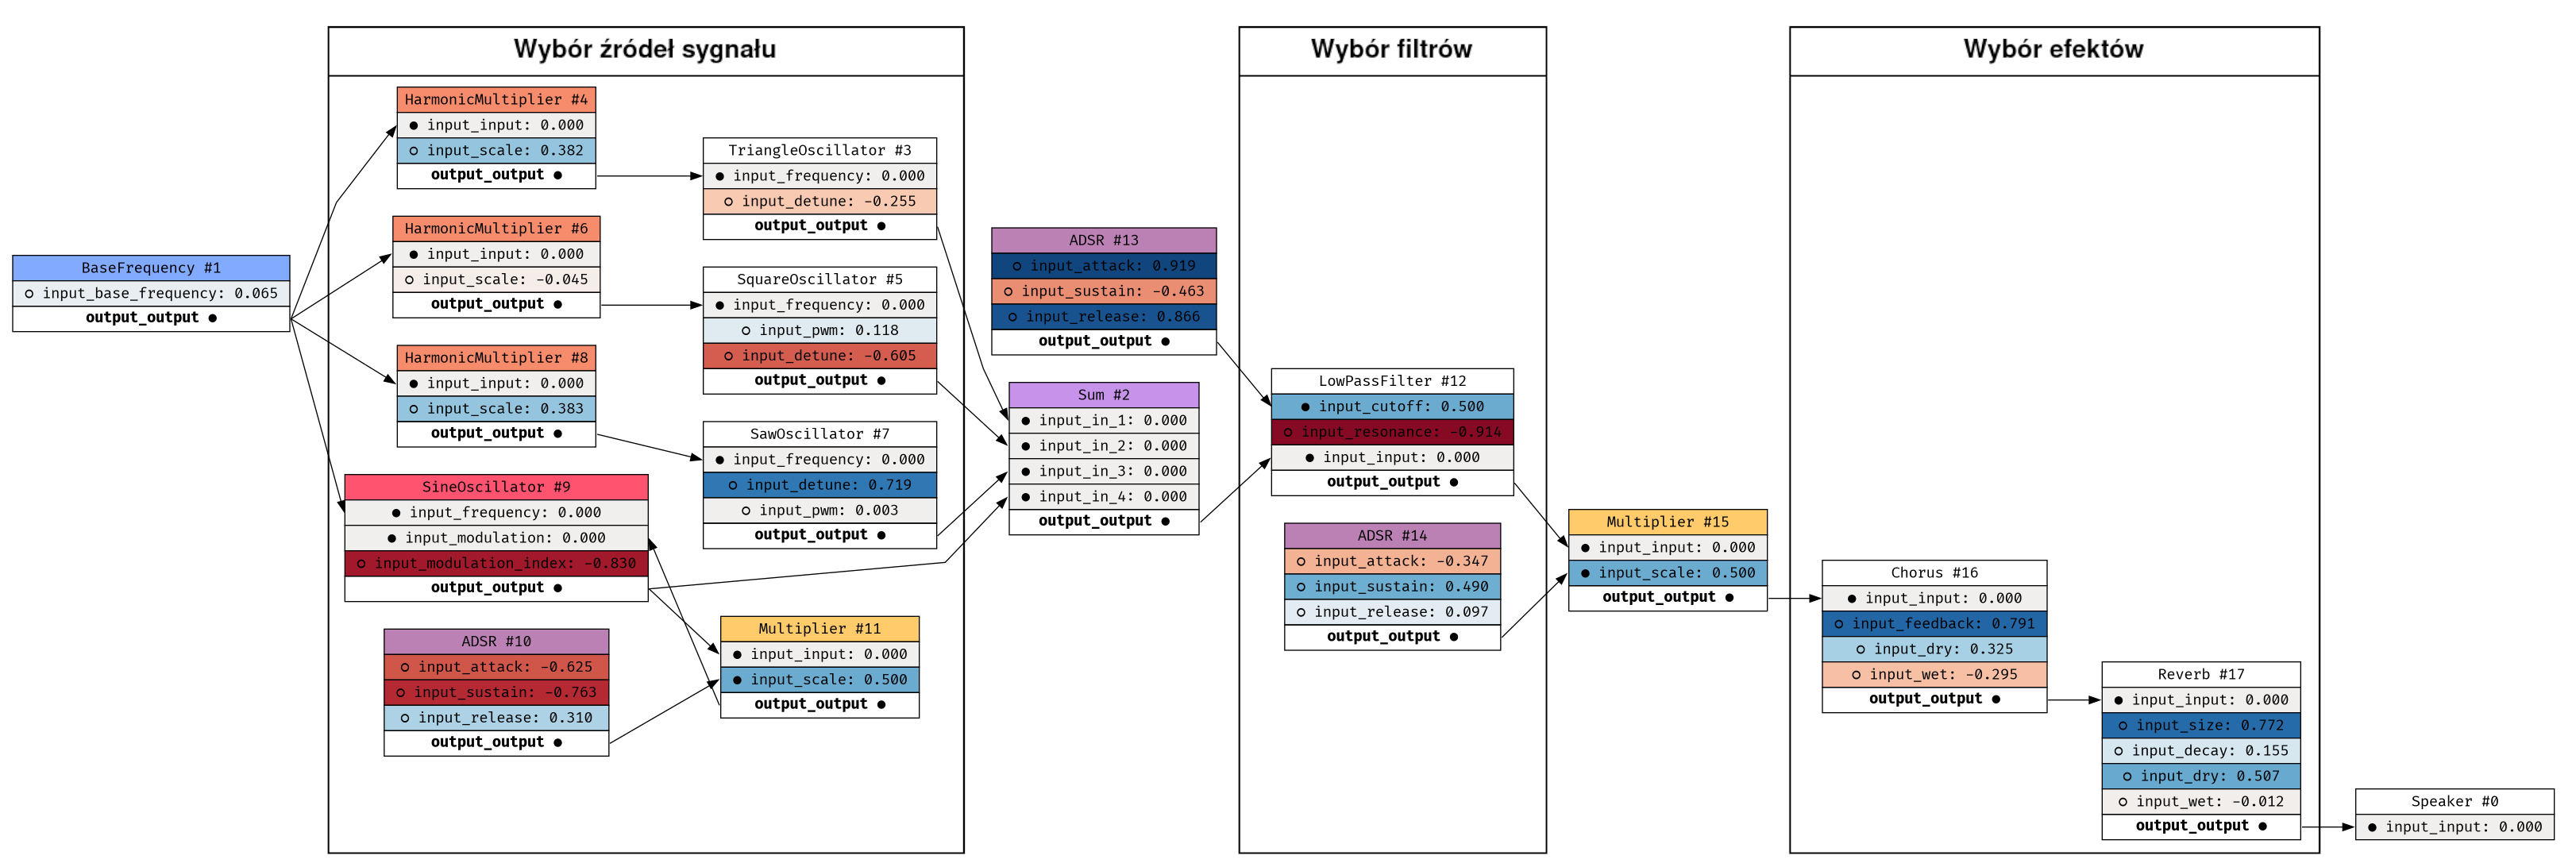
\includegraphics[width=1.0\linewidth]{rys06/example_generated_graph.png}
    \caption{
      Przykład wygenerowanej struktury grafu, oznaczono segmenty z diagramu~\ref{fig:synth_architecture_diagram}.
    }\label{fig:example_generated_graph}
\end{figure}


Przykładowo, w syntezatorach wykorzystujących syntezę typu FM~\cite{yamaha_dx7_manual}, źródłem
sygnału będą operatory wykorzystujące proste sygnały sinusoidalne, poddane modulacji częstotliwości.
Dla syntezatorów analogowych (subtraktywnych), zamiast prostych sygnałów wykorzystywane są
oscylatory generujące fale kwadratowe i piłokształtne, o dużej liczbie składowych harmonicznych.
Uzasadnia to wykorzystanie filtrów dolnoprzepustowych, które z kolei nie występują w tradycyjnych
syntezatorach FM (pojawiają się dopiero we współczesnych modelach~\cite{digitone_manual}).
Instrumenty eksperymentalne, wykorzystujące mniej popularne rodzaje syntezy, takie jak
\textit{physical modeling}~\cite{yamaha_vl1_manual}, często opierają się jedynie na rozbudowanej
sekcji oscylatorów, które posiadają wystarczająco dużo parametrów by wynagrodzić tym brak
sekcji subtraktywnej. Po drugiej stronie spektrum znajdują się instrumenty wykorzystujące
głównie sekcję efektów i syntezę granularną~\cite{microcosm_hologram_manual},
aby w nieoczekiwany sposób modyfikować proste próbki dźwięku.

\section{Wybór źródeł sygnału}

Graf posiada 3 sloty dla węzłów generujących sygnał. W pracy zaimplementowano różne
typy syntezy, które mogą być wykorzystane przez algorytm do syntezy dźwięków o różnorodnych barwach. 

\subsection{Synteza FM}

Zaimplementowane w pracy geny odpowiedzialne za syntezy FM odwzorowują uproszczone algorytmy syntezy wykorzystane
w syntezatorze \textit{Yamaha DX7}~\cite{yamaha_dx7_manual}.

\subsubsection{Gen \texttt{FM1}}

Gen \texttt{FM1}

\begin{figure}[H]
    \centering
    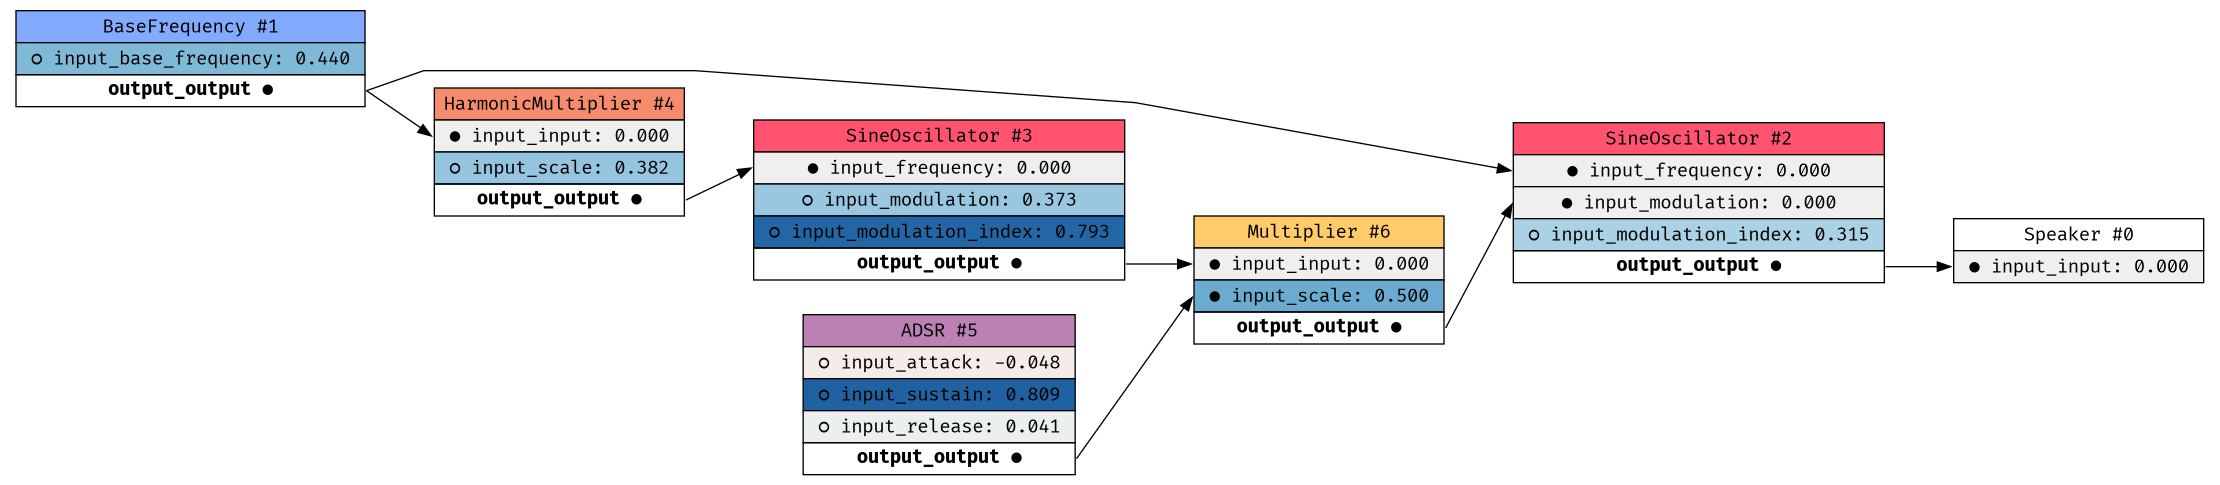
\includegraphics[width=1.0\linewidth]{rys06/gene_fm1.png}
    \caption{
      Graf wykorzystujący gen \texttt{FM1}.
    }\label{fig:gene_f1}
\end{figure}


Gen \texttt{FM1}, przedstawiony na diagramie~\ref{fig:gene_f2}, typową dla syntezy FM
modulację fali sinusoidalnej za pomocą innej fali sinusoidalnej. Taki układ umożliwia
uzyskanie dźwięków przypominających dźwięki fletu, trąbki lub dzwonków.

\subsubsection{Gen \texttt{FM2}}

\begin{figure}[H]
    \centering
    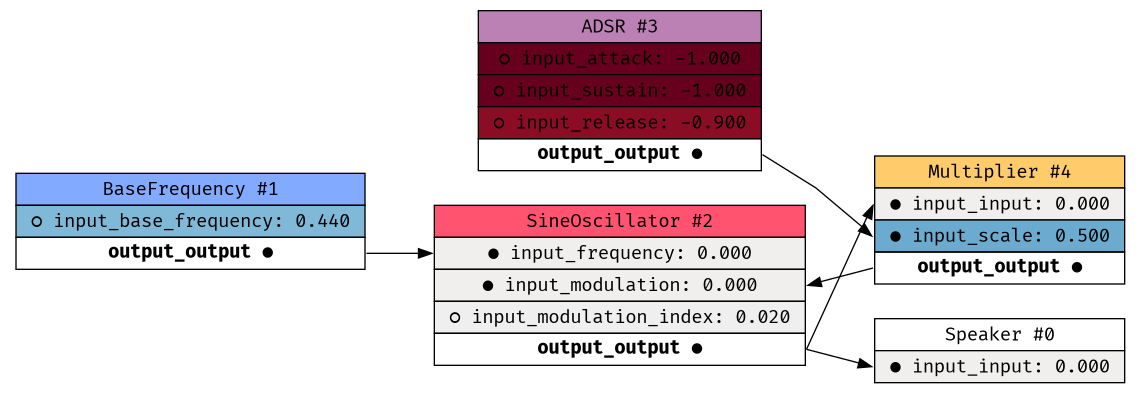
\includegraphics[width=1.0\linewidth]{rys06/gene_fm2.png}
    \caption{
      Graf wykorzystujący gen \texttt{FM2}.
    }\label{fig:gene_f2}
\end{figure}

Gen \texttt{FM2}, zilustrowany na diagramie~\ref{fig:gene_f2}, wykorzystuje pojedynczy
operator ze sprzężeniem zwrotnym. W zależności od ustawionych parametrów, taka struktura pozwala
na uzyskanie dźwięków przypominających uderzenie w strunę lub służyć jako źródło szumu.

\subsection{Synteza \textit{analog modeling}}

Zaimplementowane w pracy geny odpowiedzialne za syntezy FM odwzorowują uproszczone algorytmy syntezy wykorzystane
w syntezatorze \textit{Korg Minilogue xd}~\cite{yamaha_dx7_manual}.

\subsubsection{Gen \texttt{AN1}}

\begin{figure}[H]
    \centering
    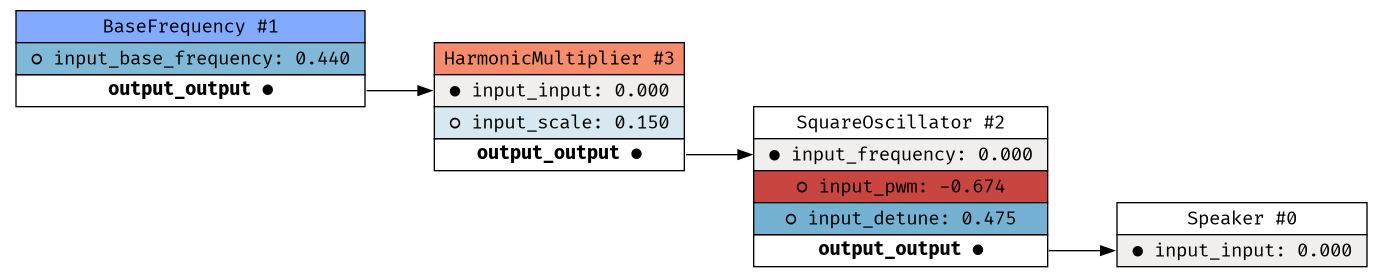
\includegraphics[width=1.0\linewidth]{rys06/gene_an1.png}
    \caption{
      Graf wykorzystujący gen \texttt{AN1}.
    }\label{fig:gene_an1}
\end{figure}

Gen \texttt{AN1} (diagram~\ref{fig:gene_an1}) pozwala na uzyskanie fal prostokątnych o różnej szerokości impulsów.


\subsubsection{Gen \texttt{AN2}}

\begin{figure}[H]
    \centering
    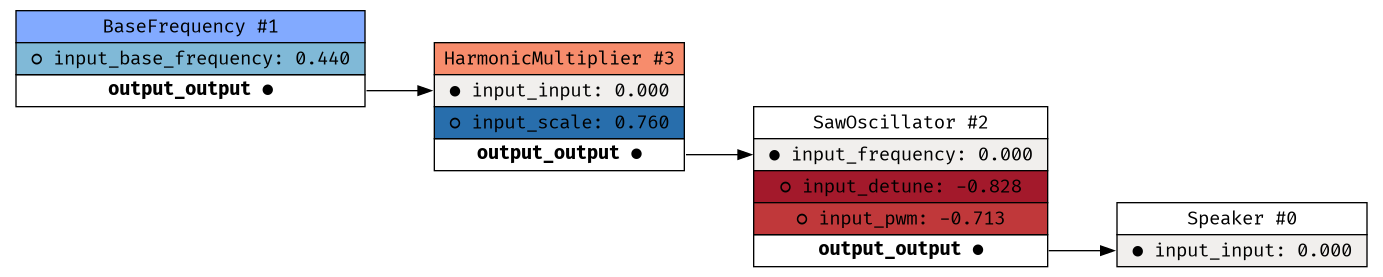
\includegraphics[width=1.0\linewidth]{rys06/gene_an2.png}
    \caption{
      Graf wykorzystujący gen \texttt{AN2}.
    }\label{fig:gene_an2}
\end{figure}

Gen \texttt{AN2}, przedstawiony na diagramie~\ref{fig:gene_an2}, pozwala na uzyskanie sygnałów piłokształtnych.


\subsubsection{Gen \texttt{AN3}}

\begin{figure}[H]
    \centering
    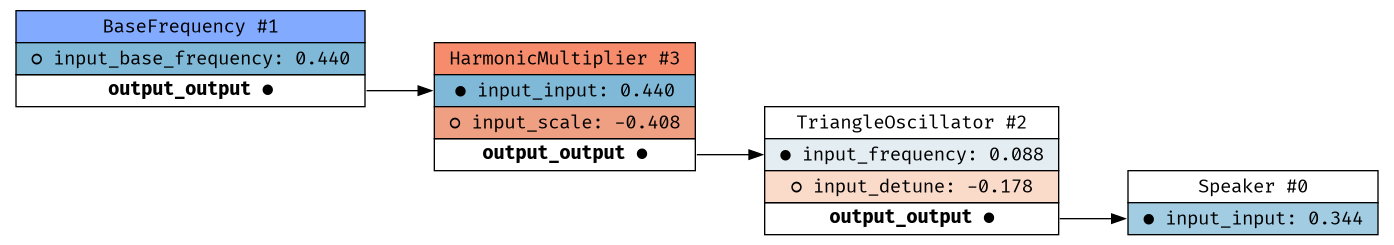
\includegraphics[width=1.0\linewidth]{rys06/gene_an3.png}
    \caption{
      Graf wykorzystujący gen \texttt{AN3}.
    }\label{fig:gene_an3}
\end{figure}

Gen \texttt{AN3}, (diagram~\ref{fig:gene_an3}), generuje sygnały trójkątne.

\section{Wybór filtrów}

W pracy wykorzystano gotową implementację filtru cyfrowego, emulującego
rezonansowy filtr drabinkowy~\cite{ladder_filter_rust}.
Implementacja została wykorzystana do wytworzenia filtrów dolno oraz górnoprzepustowego.

\section{Wybór efektów}

W pracy wykorzystano gotowy algorytm pogłosu (\textit{reverb}) oparty na~\cite{reverb}.
Algorytm generujący echo (\textit{delay}) został zaimplementowany jako bufor kołowy.
Algorym generujący efekt \textit{chorus} został zaimplementowany jako wariant algorytmu \textit{delay},
w którym długość bufora jest modulowana przez falę sinusoidalną. Efekty połączone sa w łańcuch
$chorus \rightarrow delay \rightarrow reverb$. Algorytm generacji wybiera, które efekty będą obecne w grafie.
Diagram~\ref{fig:example_generated_effects} ilustruje fragment grafu,
w którego strukturze znajdują się wszystkie 3 efekty.

\begin{figure}[H]
    \centering
    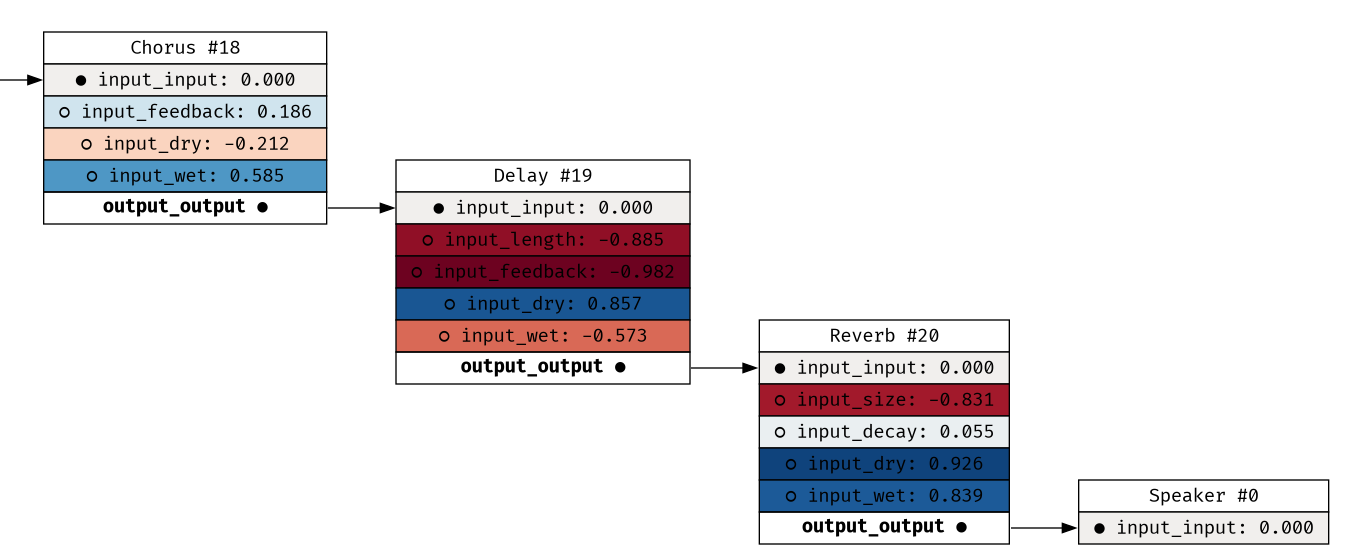
\includegraphics[width=1.0\linewidth]{rys06/example_generated_effects.png}
    \caption{
      Przykładowy łańcuch efektów w grafie.
    }\label{fig:example_generated_effects}
\end{figure}
